\documentclass[11pt,a4paper,notitlepage]{report}
\usepackage[british]{babel} % British hyphenation patterns, etc.
\usepackage{csquotes}
\usepackage[pdfusetitle,hidelinks]{hyperref}
\usepackage[titletoc]{appendix}
\usepackage[T1]{fontenc}
\usepackage{fontspec}
\usepackage[final]{microtype}
\usepackage[a4paper]{geometry}
\usepackage{listings}
\usepackage{titling}
\usepackage[style=ieee,backend=biber]{biblatex}
\usepackage{fancyvrb} % VerbatimInput
\usepackage{tabularx}
\usepackage{multirow}
%\usepackage[toc]{multitoc}
\usepackage{booktabs} % top/midrule
\usepackage{graphicx}
\usepackage{floatrow}
\usepackage{float}
\usepackage{enumitem} % noitemsep
\usepackage{tikz}
\usepackage{pgfplotstable}
\usetikzlibrary{chains,shapes,arrows,positioning,backgrounds}

\pgfplotsset{compat=1.14}

\newenvironment{changemargin}[2]{%
\begin{list}{}{%
\setlength{\topsep}{0pt}%
\setlength{\leftmargin}{#1}%
\setlength{\rightmargin}{#2}%
\setlength{\listparindent}{\parindent}%
\setlength{\itemindent}{\parindent}%
\setlength{\parsep}{\parskip}%
}%
\item[]}{\end{list}}

\renewcommand*{\bibfont}{\small}
\addbibresource{references.bib}

\lstset{basicstyle=\small\ttfamily,captionpos=b}

% Titlepage formatting
\pretitle{\begin{center}\Huge\bfseries}
\posttitle{\par\end{center}\vspace{0.5em}}
\preauthor{\begin{center}\Large}
\postauthor{\par\large\texttt{\supervisor}\end{center}}
\predate{\par\large\centering}
\postdate{\par\par}

\newcolumntype{L}{>{\ttfamily\arraybackslash}p{6em}}

% Magic hackery to automaticly generate the word count
\immediate\write18{texcount \jobname.tex -inc -1 -sum -out=wordcount.txt}
\newcommand\wordcount{\input{wordcount.txt}\unskip}

\title{Binary Code Translation from Register to Stack based code}
\author{Charles Pigott}
\date{\today}
\newcommand\supervisor{Supervisor: Dr.\ Christopher Crispin-Bailey}

\begin{document}

\maketitle

%TC:group lstlisting 0 0
\begin{abstract}
  This project aims to show that by converting code written for a simple
  register-based architecture or processor to a stack-based architecture,
  performance improvements can be found.  A review is made of the history of
  register and stack-based computing, and previous work on stack optimisation
  techniques.  A combined translator and interpreter for running register code
  on a stack machine is designed and implemented
  (\texttt{https://github.com/LordAro/reg2stack}).  Several different
  optimisation models implemented by the software are then tested, the results
  of which are evaluated.
\end{abstract}

\vfill

\small{The main body of the report (excluding the appendices) is
\wordcount~words, counted by \texttt{texcount}}

\cleardoublepage%

\normalsize
\tableofcontents

\chapter{Introduction}\label{ch:introduction}
\section{Background}
Transmeta were a US based company, who in 2000 surprised the computer
architecture industry by developing a chip which dynamically translates Intel
binary code into machine language instructions for another (highly optimised
RISC) CPU core. In doing so it allows Intel code to execute in real-time without
recompilation, but using a (claimed) much more power-efficient processor
architecture.

\section{Aims}
The objective of this project is to show that by converting code written for a
simple register-based architecture or processor to a stack-based architecture,
performance improvements can be found. This includes an implementation that can
translate code intended for a register-based architecture to run on a
stack-based architecture. Testing the output of this implementation is intended
to gain some performance related results and enable conclusions to be drawn from
them.

\section{Limitations}
Sourcing physical processors and the toolchains capable of compiling and running
code on both register-based and stack-based architectures is difficult, as
existing systems tend to be either very out of date, with only partial support,
or not exist on both platforms. Because of this, the project seeks to emulate
the architectures instead.

Since the architectures will be emulated, there are very few advantages to
continuing to use the architecture's native binary code, so this project will
instead use the respective architecture's assembly language, rather than the
binary code.

\section{Statement of Ethics}
This project has very few ethical concerns. This project only intends to
implement already published work and show that their results are correct. In
addition, Transmeta published results for their similar project over a decade
ago with their Crusoe processor and have since closed down any microprocessor
production operations and bought out, therefore any implications of the results
of this project will be unlikely to have any further affect on any commercial
businesses. There is the case of transferring the ideas from this project to
different architectures. The source architectures in this project are fully
evaluated for side effects, but changing to a different architecture may result
in different results if not examined fully, depending on the architecture. This
could cause issues for high-integrity software where correctness is crucial. The
software produced by this project has been released under a permissive
open-source licence now that it is completed, should anyone else want to take
the project any further.

\section{Problem approach}
Initially, relevant literature is reviewed, focusing on the work done by
Transmeta, but also covering computer architectures, code translation and stack
optimisation (Chapter~\ref{ch:litreview}). The knowledge from this is used to
make a list of requirements for the implentation of the translation program
(Chapter~\ref{ch:problemanalysis}). The program is then designed and
implemented, documenting the problems and solutions found along the way
(Chapter~\ref{ch:designimplementation}). The completed implementation is then
tested appropriately and results recorded and evaluated
(Chapter~\ref{ch:testingresults}). Finally, conclusions are drawn and options
for any further work set out and discussed (Chapter~\ref{ch:conclusions}).

\chapter{Literature Review}
\section{Brief history of computer architectures}
With the exception of Babbage's Analytical Engine, probably the earliest
computer architecture formerly described is that of the EDVAC (Electronic
Discrete Variable Automatic Computer), in 1945 by John von~Neumann in his
incomplete `First Draft of a Report on the EDVAC'. In it, von~Neumann described
a computer which is subdivided into six separate parts - Central Arithmetic
(CA); Central Control (CC); Memory; Input; Output and External Memory (at the
time, this was intended to be something like punched tape). These components
were described using the human nervous sytem as an analogy, with the CA, CC \&
Memory acting as associative (linking) neurons, the Input \& Output acting as
sensory \& motor neurons respectively.
Von~Neumann also wanted to keep the computer as simple as possible, so suggested
that arithmetic operations (such as add and multiply) should not be overlapped,
and performed only one digit at a time. He also noted that external input/output
should first be placed into memory, rather than directly in/out of the CC or CA.
This approach to laying out the components of a computer stuck, and the
approximate idea is still used in modern processors today.\cite{FirstDraft}

\subsection{Register machines}
In the 1950s, logic gates and switches were largely implemented using the quite
large vacuum tubes and discrete transistors. With technology improving,
integrated circuits were invented, constructing logic components using layers of
metal and oxides on polished silicon. Initially, these were only used to
implement individual logic components for computers, replacing the diodes and
resistors used before, until in 1971, Intel released the 4004 microprocessor.
It was the first commercially available fully self contained microprocessor,
with its circuitry fabricated using the new `silicon gate' technology which is
why it was able to be designed and fabricated as one chip. It's worth noting
that Intel as a company didn't have much faith in this product, opting to
instead focus on its line of memory chips and partnering with a Japanese
electronic calculator firm, Busicom, to help finance the project. Nonetheless,
the 4004 was a huge success with 4004 being produced for 10 solid years and
taking Intel to the giant in the computing world that it is
today.\cite{Aspray1997Intel}

\subsection{Stack machines}
Using stacks as part of computation has been around almost as long as computing
itself, with Zuse's Z4 making use of them for subroutines in
1945.\cite{Speiser2000KZZ} These days stacks in computer architectures and
instruction sets are nearly exclusively limited to stack frames, to give the
ability to do context ``saving'' and ``loading'' with function calls, in favour
of register based computation. However, there is a notable exception - the Java
Virtual Machine (JVM) uses a stack-based bytecode as its underlying programming
language.\cite{Schoeberl2005Design}

Instead of having named registers to store values as part of computations, stack
machines use a stack data structure


stack scheduling


\section{Binary Translation}
ibm binary translation

transputer

\subsection{Transmeta Crusoe}
In 2000, Transmeta published a thing which was interesting\cite{TransmetaCodeMorph}



\chapter{Problem Analysis}\label{ch:problemanalysis}
The program implementation should be broken down into a number of steps. First
will be deciding on the source (register) and target (stack) architectures.  The
first part of the implementation will be to implement emulators for the chosen
architectures.  Some conversion routines for register to stack architectures
will be then implemented. After this, the generated stack code will have
optimisation techniques applied to it. Finally, suitable test programs will be
written.

\section{Requirements}
The following is a codified list of required features for the implementation of
the project:

\begin{itemize}[noitemsep]
  \item Fully functioning emulator for a register machine architecture
  \item Fully functioning emulator for a stack machine architecture
  \item Ability to generate stack code from register code
\end{itemize}

There are also a certain number of desirable features that are medium priority.
If these are not implemented, they will be discussed in the further work section (Section~\ref{sec:furtherwork})

\begin{itemize}[noitemsep]
  \item Peephole optimisations on generated stack code
  \item Koopman-style optimisations on generated stack code
\end{itemize}

There are also a few ``nice-to-have'' features, that are low priority and not
all that important for the project to be deemed a `success'.

\begin{itemize}[noitemsep]
  \item Translation threshold --- like the TransMeta implementation, only
  translate regions of code if they are executed more than a certain number of
  times.
  \item Ability to more easily visualise differences between handwritten and
  generated code, e.g.\ graphs or running side-by-side.
\end{itemize}

\chapter{Design and Implementation}\label{ch:designimplementation}

An early decision to be made was to write emulators for the register \& stack
machines chosen. Toolchains for `obscure' architectures such as the ones likely
to be chosen tend to be rather limited in nature and either out-of-date, broken
or both. Writing emulators for the architectures creates extra programming
work, but means that the choices of programming language and style are much
greater.

It was then decided that to simplify the design, the program would be interpret
assembly source code of the register \& stack architectures instead of running
the compiled binary. Doing it this way is only an abstraction over actually
reading the binaries, and skips out having to compile the source code and then
decode it again. Relatively speaking, it would not be difficult to make a
program that does this but was deemed unnecessary for the core part of this
project, converting a register-based instruction set to a stack-based one.

\section{Programming language choice}
C++ is a systems programming language that is well known for it's hugely
powerful templates for generic programming, its ability to use multiparadigm
styles of programming and its high speed, with significant work being put into
optimising compilers for the language. Using object-orientated-programming, the
conversion routines can be built on top of one of the emulators, with little
duplication of code.

C++ does have some disadvantages however. Its (relatively) low-level nature and
power makes it easy to make errors in programming and logic, and its compiler
errors for templates are infamous for taking up many pages. In fact, C++'s own
creator has been quoted as saying ``C makes it easy to shoot yourself in the
foot; C++ makes it harder, but when you do it blows your whole leg off'' when
comparing C++ to its parent language C. That said, modern C++ has been making
big improvements to the language since 2011, with smart pointers, lambdas \&
type deduction fixing many of the language's major criticisms.

Some thought was put into other higher-level languages, such as Python, but as
these languages are interpreted instead of compiled, they incur an inherent
speed penalty by comparison which with a speed sensitive project such as this
where the emulators need to complete executing instructions in a specified
amount of time is not a thing that is desirable to be worrying about.

With all this in mind, it was decided that existing familiarity with the C++
language was important as were the benefits of not having to worry about the
speed of the emulators themselves for development outweighed the disadvantages.

\section{Architecture choices}
An immediate shortlist of register architectures was drawn up, of the Z80, the
Picoblaze, and the DCPU-16.

The Zilog Z80 is a microprocessor introduced in 1976. It is 8-bit based with the
capability to address 64KB of memory by means of combining its registers. An
extremely popular processor during the 1980s, it is still produced to this day
for uses in embedded systems. It has its own assembly language that has both
register and stack elements. Xilinx's Picoblaze is a `soft processor core',
meaning that isn't manufactured specially, rather is fabricated on an FPGA
(field-programmable gate array) by the user. It uses an 8-bit RISC architecture,
which makes it very simple to fabricate and run. The DCPU-16 isn't actually a
real processor, and has never been produced. It is the invention of Markus
Persson to be emulated as part of a game he was creating that never ended up
getting finished, but there was significant interest in it, which means that
there was many programs and emulators produced for the processor regardless.
It's a 16-bit processor that has modularity in mind in the architecture --- the
computer would `connect' to peripherals to do its IO instead of a more common
console output interface.

\noindent\begin{minipage}{0.5\textwidth}
\begin{lstlisting}[caption={Z80 ASM},captionpos=b]
      LD a, 0
      LD (CURCOL), a
      LD (CURROW), a
      LD hl, text
      B_CALL(_PutS)
      RET
text:
      .db "Hello, world!", 0
\end{lstlisting}%
\end{minipage}%
\noindent\begin{minipage}{0.5\textwidth}
\begin{lstlisting}[caption={Picoblaze ASM},captionpos=b]
module hello_world ;

initial begin
  $display ("Hello, world!");
  #10 $finish;
end

endmodule
\end{lstlisting}%
\end{minipage}

\begin{lstlisting}[caption={DCPU-16 ASM},captionpos=b]
; Attach screen
SET A, 0
SET B, vram
HWI 0

SET J, 0

:loop
SET I, vram
ADD I, J
ADD [I], 0x2000
ADD J, 1
IFN J, 12
    SET PC, loop

:crash
SET PC, crash

:vram
DAT "Hello, world!", 0
\end{lstlisting}%

As the Picoblaze is a soft-processor, it is separated into its ASM and Verilog
components and you have to connect the processor's `wires' together yourself. It
was decided that this would be too much boilerplate to be worth the effort, so
the Picoblaze was discounted. After some initial emulator implementation for the
Z80 processor, it was found that its ability to combine registers were not easy
to implement in a good way in C++, so after some thought it was decided to
continue with the DCPU-16 assembly language, after cutting it down to get rid of
the peripherals part of the language which isn't necessary for this project.

In terms of stack architectures, Forth, JVM bytecode, and J5 were shortlisted.

Forth is a very early programming languages that dates from 1970, when stack
machines were still common in everyday computing. It's a very simple compiled
language that still finds uses today in embedded systems due to how easy it is
to port to new systems, and its low memory overhead. J5 is a teaching stack
language to introduce people to stack machines and their respective languages
and it is very simple in that regard, drawing on ideas from various different
actual stack languages.

\noindent\begin{minipage}{0.5\textwidth}
\begin{lstlisting}[caption={Forth ASM},captionpos=b]
CR .( Hello, world!)
\end{lstlisting}
\end{minipage}%
\noindent\begin{minipage}{0.5\textwidth}
\begin{lstlisting}[caption={J5 ASM},captionpos=b]
OUT "Hello, world!"
\end{lstlisting}
\end{minipage}

\section{Emulator implementation}

instruction cut down



\chapter{Testing, Results and Evaluation}\label{ch:testingresults}
\section{Testing}
Due to the emulated nature of the implementation of this project, metrics such
as the time programs take to complete and power usage are fairly meaningless or
impossible to measure. Instead testing will focus on the instructions of the
original register-based programs and stack programs that they produce, at all
levels of optimisation --- no optimisations, peephole optimisations, and
stack-scheduling.

The results will be looking to find the relationship between the number of
register instructions to generated instructions, so that the effect of each
optimising level can be assessed. Further attention will be paid to the number
of memory accesses made by the stack program, as stack-scheduling is supposed to
be able to significantly reduce redundant memory accesses produced by emulating
registers as memory.

Using a simple memory model, a basic figure for ``program cost'' can be
produced. While there will be no equivalent available for the source
register-based programs, it will be beneficial to see the difference between
each optimisation level. The memory model can also be used to measure the effect
of the translation cache, by giving the conversion and caching of the register
code an (estimated) high cost, to simulate the effects of not having to
convert heavily used loops many times over.

Testing will be done using a series of programs handwritten for the DCPU-16
emulator. For testing purposes, simple test programs (called \texttt{simple},
\texttt{loop} and \texttt{redundant}) were created only to test compiler
correctness and were not used for benchmarking.

For the actual benchmark programs, there are several desirable features to
consider. Since stack-scheduling is an intra-block algorithm, the benchmark
programs should vary between types of loops that are used, and their frequency
of use. Highly used loops do well to test the translation cache system. The
programs should also use a wide variety of register instructions to achieve
better coverage of the translator and emulators.

A common set of tests used for these type of the programs is the Standford
Benchmark Suite\cite{stanford}. It's a set of programs written in C that are
fairly short in code and execution time. It also has the advantage of not
requiring any input, which both the source DCPU-16 and J5 instruction sets lack.
Examples of programs in it include bubble sort, towers of hanoi and a matrix
multiplication.

However, since the implementation in this project lacks any sort of subroutine
or function support, many of the programs would be quite difficult to feasibly
implement. With that in mind, a different set of benchmarks was created. Given
more time, further benchmarks would have been created so as to produce more
raw data, for better results.

\begin{itemize}[noitemsep]
  \item \texttt{bsort} --- Bubble sort benchmark. Sorts 32 integers and prints
  the result
  \item \texttt{fib20} --- Calculates and prints the first 20 fibonacci numbers
  \item \texttt{primes} --- Uses a prime sieve to get all the prime numbers up
  to 100
  \item \texttt{tri100} --- Outputs the first 100 triangle numbers, using the
    addition formula
\end{itemize}

With the above in mind, the above four programs were written in DCPU-16
assembly. They were chosen as reasonable examples that cover a range of
mathematical functions but in particular they vary in their use of loops, which
is the primary target of the optimisations, stack-scheduling especially. Their
contents can be seen in full in Appendix~\ref{ch:benchmarkprograms}. Notably,
\texttt{fib20} and \texttt{tri100} are similar in that they don't branch very
much, they essentially have a single loop and stay within it. The \texttt{bsort}
program is made up of several nested loops, as is \texttt{primes}, however it is
written in such a way that the loops are not nested within the code, which makes
it jump around a lot more.

\section{Results}

\begin{table}
  \begin{tabular}{r r r r}
                    &   Base & Peephole & Koopman \\ \toprule
    \texttt{bsort}  &  24024 &    22343 &   22233 \\ \midrule
    \texttt{fib20}  &    665 &      608 &     606 \\ \midrule
    \texttt{primes} &   6717 &     6619 &    6619 \\ \midrule
    \texttt{tri100} & 111381 &   106332 &  106332 \\ \midrule
  \end{tabular}
  \caption{No.\ of instructions executed}\label{tab:instructions}
\end{table}

\begin{table}
  \begin{tabular}{r r r r}
                    &  Base & Peephole & Koopman \\ \toprule
    \texttt{bsort}  &  7792 &     6703 &    6065 \\ \midrule
    \texttt{fib20}  &   234 &      196 &     175 \\ \midrule
    \texttt{primes} &  1912 &     1912 &    1643 \\ \midrule
    \texttt{tri100} & 35345 &    35345 &   30296 \\
  \end{tabular}
  \caption{No.\ of LOAD/STORE instructions executed}\label{tab:meminstructions}
\end{table}

\pgfplotstableread[col sep=comma,header=false]{%
bsort,24024,22343,22233
fib20,665,608,606
primes,6717,6619,6619
tri100,111381,106332,106332
}\tracedata%

\pgfplotstableread[col sep=comma,header=false]{%
bsort,7792,6703,6065
fib20,234,196,175
primes,1912,1912,1643
tri100,35345,35345,30296
}\tracememdata%

\pgfplotsset{%
  relative series/.style={%
    table/y expr=\thisrow{#1}/\thisrow{1},
    table/meta=#1
  },
  relative graph/.style={%
    width=13cm,
    ymajorgrids=true,
    major x tick style = transparent,
    major y tick style = transparent,
    scaled y ticks = false,
    ybar=0pt,
    ymin=0.5,
    bar width=0.75cm,
    enlarge x limits=0.2,
    symbolic x coords={bsort,fib20,primes,tri100},
    xtick=data,
    legend cell align=left,
    legend style={%
      at={(1,0)},
      anchor=south west,
      column sep=1ex
    }
  }
}

\begin{figure}
  \begin{tikzpicture}
    \begin{axis}[relative graph]
      \addplot table [relative series=1] {\tracedata};
      \addplot table [relative series=2] {\tracedata};
      \addplot table [relative series=3] {\tracedata};
      \legend{Base,Peephole,Koopman}
    \end{axis}
  \end{tikzpicture}
  \caption{Relative no.\ of instructions executed}\label{fig:relativeinstructions}
\end{figure}

\begin{figure}
  \begin{tikzpicture}
    \begin{axis}[relative graph]
      \addplot table [relative series=1] {\tracememdata};
      \addplot table [relative series=2] {\tracememdata};
      \addplot table [relative series=3] {\tracememdata};
      \legend{Base,Peephole,Koopman}
    \end{axis}
  \end{tikzpicture}
  \caption{Relative no.\ of LOAD/STORE instructions executed}\label{fig:relativememinstructions}
\end{figure}

Tables~\ref{tab:instructions} \&~\ref{tab:meminstructions} represent the number
of instructions executed for a complete run of the benchmark programs, and the
number of LOAD/STORE operations for each of them for the same run, respectively.
Figures~\ref{fig:relativeinstructions} \&~\ref{fig:relativememinstructions}
graph the relative decrease in the number of instructions executed for each
optimisation level, where no optimisations is the base level at one.

\begin{table}
\begin{tabular}{l l r r r r}
  Program & Block & Register & Stack & Peephole & Koopman \\ \toprule
  \multirow{6}{*}{\texttt{bsort}}  & & 34 & 103 & 102 & 102 \\
  & \texttt{LOOP}                    &  2 &   9 &   8 &   8 \\
  & \texttt{LOOP2}                   &  5 &  25 &  24 &  24 \\
  & \texttt{SWAP}                    &  3 &  24 &  24 &  23 \\
  & \texttt{POST}                    &  6 &  27 &  25 &  25 \\
  & \texttt{RESL}                    &  4 &  22 &  21 &  21 \\ \midrule
  \multirow{2}{*}{\texttt{fib20}}  & &  6 &  34 &  32 &  32 \\
  & \texttt{LOOP}                    &  7 &  20 &  20 &  18 \\ \midrule
  \multirow{5}{*}{\texttt{primes}} & &  2 &   6 &   6 &   6 \\
  & \texttt{LOOP}                    &  2 &  12 &  12 &  12 \\
  & \texttt{SCANNED}                 &  4 &  17 &  16 &  16 \\
  & \texttt{SCAN}                    &  3 &  17 &  17 &  17 \\
  & \texttt{LOOP2}                   &  4 &  24 &  24 &  24 \\ \midrule
  \multirow{5}{*}{\texttt{tri100}} & &  2 &   6 &   6 &   6 \\
  & \texttt{LOOP}                    &  2 &   6 &   6 &   6 \\
  & \texttt{LOOP2}                   &  4 &  20 &  19 &  19 \\
  & \texttt{BREAK}                   &  4 &  23 &  22 &  22 \\
\end{tabular}
\caption{Instruction counts per block}\label{tab:instructionperblock}
\end{table}

\pgfplotstableread[col sep=comma]{%
Register,Stack,Peephole,Koopman
%34,103,102,102
2,9,8,8
5,25,24,24
3,24,24,23
6,27,25,25
4,22,21,21
6,34,32,32
7,20,20,18
2,6,6,6
2,12,12,12
4,17,16,16
3,17,17,17
4,24,24,24
2,6,6,6
2,6,6,6
4,20,19,19
4,23,22,22
}\blockdata%

\begin{figure}
  \begin{tikzpicture}
    \begin{axis}[
        xlabel=No.\ of register instructions,
        ylabel=No.\ of stack instructions,
        legend cell align=left,
        legend style={%
          at={(1,0)},
          anchor=south west,
          column sep=1ex
        }
    ]
      \addplot [only marks,mark=x,blue] table [y=Stack] {\blockdata};
      \addplot [thick,blue] table [y={create col/linear regression={y=Stack}}] {\blockdata};
      \addlegendentry{Base}
      \addplot [only marks,mark=x,red] table [y=Peephole] {\blockdata};
      \addplot [thick,red] table [y={create col/linear regression={y=Peephole}}] {\blockdata};
      \addlegendentry{Peephole}
      \addplot [only marks,mark=x,brown] table [y=Koopman] {\blockdata};
      \addplot [thick,brown] table [y={create col/linear regression={y=Koopman}}] {\blockdata};
      \addlegendentry{Koopman}
      \legend{Base,,Peephole,,Koopman}
    \end{axis}
  \end{tikzpicture}
  \caption{Graph of register blocks to stack equivalents}\label{fig:instructionperblock}
\end{figure}

Table~\ref{tab:instructionperblock} lists the number of stack instructions
produced per block of register code, for different optimisation levels. The
`empty' block row represents the initial block of the program, with no label. It
is graphed in Figure~\ref{fig:instructionperblock}. Notably for the graph, the
initialisation block for \texttt{bsort} is omitted as it is considerably larger
than anything else and considered anomalous.

\begin{table}
\begin{tabular}{l l r r r r}
  Program & Block & Register & Stack & Peephole & Koopman \\ \toprule
  \multirow{6}{*}{\texttt{bsort}}  & & 34 & 35 & 34 & 34 \\
  & \texttt{LOOP}                    &  2 &  3 &  3 &  3 \\
  & \texttt{LOOP2}                   &  5 &  8 &  7 &  6 \\
  & \texttt{SWAP}                    &  3 & 10 & 10 &  9 \\
  & \texttt{POST}                    &  6 &  6 &  5 &  5 \\
  & \texttt{RESL}                    &  4 &  6 &  6 &  5 \\ \midrule
  \multirow{2}{*}{\texttt{fib20}}  & &  6 &  6 &  6 &  4 \\
  & \texttt{LOOP}                    &  7 & 12 & 11 &  9 \\ \midrule
  \multirow{5}{*}{\texttt{primes}} & &  2 &  2 &  6 &  2 \\
  & \texttt{LOOP}                    &  2 &  2 &  2 &  2 \\
  & \texttt{SCANNED}                 &  4 &  4 &  5 &  3 \\
  & \texttt{SCAN}                    &  3 &  5 &  4 &  5 \\
  & \texttt{LOOP2}                   &  4 &  7 &  7 &  6 \\ \midrule
  \multirow{5}{*}{\texttt{tri100}} & &  2 &  2 &  2 &  2 \\
  & \texttt{LOOP}                    &  2 &  2 &  2 &  2 \\
  & \texttt{LOOP2}                   &  4 &  7 &  7 &  6 \\
  & \texttt{BREAK}                   &  4 &  5 &  5 &  4 \\
\end{tabular}
  \caption{LOAD/STORE instruction counts per block}
\label{tab:meminstructionperblock}
\end{table}


\pgfplotstableread[col sep=comma]{%
Register,Stack,Peephole,Koopman
%34,35,34,34
2,3,3,3
5,8,7,6
3,10,10,9
6,6,5,5
4,6,6,5
6,6,6,4
7,12,11,9
2,2,6,2
2,2,2,2
4,4,5,3
3,5,4,5
4,7,7,6
2,2,2,2
2,2,2,2
4,7,7,6
4,5,5,4
}\blockmemdata%

\begin{figure}
  \begin{tikzpicture}
    \begin{axis}[
        xlabel=No.\ of register instructions,
        ylabel=No.\ of LOAD/STORE stack instructions,
        legend cell align=left,
        legend style={%
          at={(1,0)},
          anchor=south west,
          column sep=1ex
        }
    ]
      \addplot [only marks,mark=x,blue] table [y=Stack] {\blockmemdata};
      \addplot [thick,blue] table [y={create col/linear regression={y=Stack}}]
      {\blockmemdata};
      \addlegendentry{Base}
      \addplot [only marks,mark=x,red] table [y=Peephole] {\blockmemdata};
      \addplot [thick,red] table [y={create col/linear regression={y=Peephole}}]
      {\blockmemdata};
      \addlegendentry{Peephole}
      \addplot [only marks,mark=x,brown] table [y=Koopman] {\blockmemdata};
      \addplot [thick,brown] table [y={create col/linear regression={y=Koopman}}]
      {\blockmemdata};
      \addlegendentry{Koopman}
      \legend{Base,,Peephole,,Koopman}
    \end{axis}
  \end{tikzpicture}
  \caption{Graph of register blocks to stack memory read/writes}
\label{fig:meminstructionperblock}
\end{figure}

Table~\ref{tab:meminstructionperblock} lists the number of LOAD/STORE
instructions produced per block of register code, for different optimisation
levels. Similarly to previous tables, the `empty' block row represents the
initial block at the start of the program, given it has no label. The table is
graphed in Figure~\ref{fig:meminstructionperblock} and again excludes the
initialisation block for \texttt{bsort}. Note that the table and figure compare
against the total register instruction count, rather than the number of memory
usages the register blocks have. This is because as registers are being emulated
as memory positions, it would be difficult to reliably determine which register
instructions either use or cause memory usages.

\begin{table}
  \begin{tabular}{l l}
    Caching a block & 10 $\times$ number of register instructions \\
    Retrieving a block & 1 \\
    Memory accesses & 3 \\
    Branches & 2 \\
    Other & 1 \\
  \end{tabular}
  \caption{Memory model used for estimating program cost}\label{tab:memmodel}
\end{table}

\begin{table}
  \begin{tabular}{r r r r}
                    &   Base & Peephole & Koopman \\ \toprule
    \texttt{bsort}  &  97292 &    93746 &   92454 \\ \midrule
    \texttt{fib20}  &   1300 &     1224 &    1142 \\ \midrule
    \texttt{primes} &  19615 &    19516 &   18978 \\ \midrule
    \texttt{tri100} & 202089 &   197040 &  186942 \\ \midrule
  \end{tabular}
  \caption{Program cost with caching disabled}\label{tab:costnocaching}
\end{table}

\begin{table}
  \begin{tabular}{r r r r}
                    &   Base & Peephole & Koopman \\ \toprule
    \texttt{bsort}  &  40902 &    37356 &   36064 \\ \midrule
    \texttt{fib20}  &   1300 &     1224 &    1142 \\ \midrule
    \texttt{primes} &  11981 &    11882 &   11344 \\ \midrule
    \texttt{tri100} & 192583 &   187534 &  177436 \\ \midrule
  \end{tabular}
  \caption{Program cost with caching}\label{tab:costcaching}
\end{table}

\pgfplotstableread[col sep=comma,header=false]{%
bsort,97292,93746,92454,40902,37356,36064
fib20,1300,1224,1142,1300,1224,1142
primes,19615,19516,18978,11981,11882,11344
tri100,202089,197040,186942,192583,187534,177436
}\costdata%

\begin{figure}
  \begin{tikzpicture}
    \begin{axis}[relative graph,bar width=0.25cm,ymin=0]
      \addplot table [relative series=1] {\costdata};
      \addplot table [relative series=4] {\costdata};
      \addplot table [relative series=2] {\costdata};
      \addplot table [relative series=5] {\costdata};
      \addplot table [relative series=3] {\costdata};
      \addplot table [relative series=6] {\costdata};
      \legend{Base,Base Cached,Peephole,Peephole Cached,Koopman,Koopman Cached}
    \end{axis}
  \end{tikzpicture}
  \caption{Relative program cost with and without caching}\label{fig:progcost}
\end{figure}

Tables~\ref{tab:costnocaching} \&~\ref{tab:costcaching} describe the `costs' of
running the benchmarking programs with the memory model described in
Table~\ref{tab:memmodel}. The two tables are represented in
Figure~\ref{fig:progcost}.

\section{Evaluation}\label{sec:testingevaluation}
The basic results (Seen in Table~\ref{tab:instructions} and
Figure~\ref{fig:relativeinstructions}) are somewhat counterintuative, showing
that the Peephole optimisation stage does the bulk of the the overall executed
instruction count reduction and that Koopman-style stack scheduling has very
little effect.

However, looking at the number of memory reads \& writes (with \lstinline{LOAD}
\& \lstinline{STORE} respectively) in Table~\ref{tab:meminstructions} (and
visualised in Figure~\ref{fig:relativememinstructions}) shows a different
result, with stack scheduling doing as much reduction as peephole optimisation
if not more, particularly in the case of the \texttt{primes} \& \texttt{tri100}
programs which have no instruction decrease with stack scheduling, but a
significant decrease in memory usage.

While the optimisation results are good (30\% reduction in memory usage is
quite substantial), it is not the same as promised by Koopman in his original
paper. Koopman claimed to be able to remove 90--100\% of redundant local
variable accesses. The results here are not quite the same measurement, but it
is hard to believe that they are the same number which is difficult to
programatically calculate --- Koopman did it by studying the program's output by
hand. It is possible that the results are so different due to the programs used
--- `tight loops' that don't make much use of variable accesses won't have as
many opportunities for stack scheduling as others.

Looking at Table~\ref{tab:instructionperblock} and its linked
Figure~\ref{fig:instructionperblock}, it can be seen that per block that while
stack-scheduling does have an effect on instruction count, it is the preliminary
peephole optimisations that have the majority of the effect. Despite this,
looking at Table~\ref{tab:meminstructionperblock} and
Figure~\ref{fig:meminstructionperblock} again shows where stack-scheduling
becomes relevant and useful with the reduction in memory usage, where the linear
regression line shows significantly lower average memory usage than peephole (\&
no) optimisations. The linear regression line for peephole optimisations starts
above the base stack output, this is likely due to the small size of the data
set --- overall the line's gradient is shallower than the base output, implying
that the results would continue to improve for larger block sizes.

Figures~\ref{fig:instructionperblock} \&~\ref{fig:meminstructionperblock} also
show the relationship of register instructions to stack instructions quite well,
with 1 register instruction generating between 4 \& 5 stack instructions
depending on the optimisation level. The memory accesses are even more
interesting, with Koopman's stack scheduling getting the ratio of register
instructions to memory accesses down to just over 1. It would be reasonable to
conclude then that the stack-scheduling does in fact remove many of the
unnecessary memory accesses.

The affects of the instruction snippet cache are more impressive. As seen
Figure~\ref{fig:progcost} (with raw data in Tables~\ref{tab:costnocaching}
\&~\ref{tab:costcaching}), each optimisation level decreases cost in a similar
fashion to the raw instruction counts discussed earlier. However, caching these
instruction blocks leads to some significant decreases in program cost for
highly looping programs, like \texttt{bsort} \& \texttt{primes}. Caching notably
has no effect on \texttt{fib20} and hardly any on \texttt{tri100} --- this is
down to the simplicity of the programs involved as they make very little use of
branching to change to a different block, only branching within the block is
used. While the costs of each instruction are only estimates
(Table~\ref{tab:memmodel}), it shows the potential effectiveness of the
instruction caching well. The estimated cost of converting register instructions
is likely quite high compared to reality, so further improvements may be
available depending on its actual efficiency.

Overall, this is a very positive result, as while the generated stack programs a
lot larger in instruction count, the memory usages are approximately equivalent.
Which, when taking into account how a stack machine would be simpler than a
similar register machine and so would be easier to construct and potentially run
at a higher clock speed, making the machines even more equivalent in program
execution cost. A reasonable continuation of this would be to alter the stack
assembly language to help remove some common repeated instruction groups. For
example, for the J5 assembly language, it would be useful to have a
\texttt{LOAD} instruction that actually took a memory address, and similarly for
the \texttt{STORE}, to save having to hardcode a separate \texttt{SET}
instruction to put a value onto the stack for each instruction. A further
advanced step would be to vary the produced stack code depending on its
contents, if a particular group of register instructions could be replaced with
something simpler than the ``standard'' generated code. A simple example of that
in this project is the peephole optimisation done on converting \texttt{SET 1}
\& \texttt{ADD} instructions to an \texttt{INC} instruction. It's not done at
the initial translation, and the register instruction set lacks a similar
instruction.

\subsection{Completion of requirements}
All key features of the project were completed, but only one of the desirable
features was able to be partially implemented, largely due to time constraints.

Requirements~\ref{itm:register} \&~\ref{itm:stack} (implementing the emulators)
were both fully implemented, with working parsers for their respective assembly
languages and able to interpret and execute any program in that language, with a
fully implemented instruction set.
Code generation was also fully implemented (Requirement~\ref{itm:generate}) that
was free of side effects.
The two key optimisation methods (Requirement~\ref{itm:optimise}) were
also implemented, including commandline flags to enable/disable them when
required (similarly to optimise flags in C++ compilers)
These flags were used to get several sets of results
(Requirement~\ref{itm:results}) focusing on length of generated code with each
optimisation level, and the number of memory accesses they did.

Unfortunately, the additional requirements (notably
Requirements~\ref{itm:moreoptimise} \&~\ref{itm:visualise}) were not able to be
implemented, largely due to time constraints on the project. While the tool did
have various debugging levels for which to get output out of, the interface was
rather crude and the data output needed some transformations (using a python
testing interface and \texttt{grep}) to get meaningful results out of, so it
would've been preferrable to have nicer interfaces. However, there was partial
completion of Requirement~\ref{itm:caching}, in that each converted block was
cached, but there was no concept of a `threshold' at which to convert them. This
would've been useful as the expense of converting and caching the initalisation
routines (that set all the input data) is likely too much compared to just
running them, bringing up the `program cost' of the program as discussed in the
results above. It would be preferable to only convert \& cache loops that are
executed lots of times.

\subsection{Program correctness}
No significant automated testing of the implementation has been done. Instead
the program's output was verified ``by eye'' and for the test run the multiple
executions were compared against each other, to ensure consistent results.

\subsection{Code quality}
The code itself is relatively extensible for future work. It is published as
open-source software at \texttt{github.com/LordAro/reg2stack} enabling any
future work to be able to be built on top of this software. The peephole
optimsation implementation allows for easy additions --- just add the relevant
function and add the function name to the list of existing functions.

Documentation of the code could definitely be improved. While complicated code
generally has comments explaining exactly why it does what it does, it's by no
means complete and could certainly be expanded. Many functions are also missing
`doccoments', which generally take the form of comments above the function
definition which can then be parsed by some external tool to generate more
formal documentation. If this were expanded it would be really helpful to future
work done on the program.

\chapter{Conclusions}\label{ch:conclusions}
In conclusion, this project was successful in its aim of finding performance
improvements in generated stack code from the na{\"\i}ve model of doing so. A
variety of optimisation techniques can be applied to the generated code to
both reduce raw instruction count and reduce memory usages. The results vary
depending on the program, but the results for this project resulted in around a
10\% decrease in raw stack instruction count and up to 25\% decrease in number
of memory accesses. More significant results were seen with conversion block
caching, seeing an up to 60\% decrease in relative program cost based on an
estimated memory model.

\section{Further work}\label{sec:furtherwork}
There is much further work that can be applied to this project.

First and foremost would be to implement further optimisations, such as the
inter-block algorithm by Bailey and the refinements done by Shannon show great
potential for further improvements especially with the tight loops of the
programs tested in this project.

There's also further scope for improving the instruction block caching system.
Other than improving how blocks are divided up, making use of Transmeta's
`translation threshold' method could prove more effective for reducing the
relative cost of running a program.

Other options would be to more properly prove that the implementation of the
emulators, and the conversion routines is correct. Formal methods to
mathematically prove correctness could even be used if so inclined. This could
be taken further to automatically generate test programs that try to break the
conversion or the emulators, generally referred to as ``fuzz testing''



\addcontentsline{toc}{chapter}{Bibliography}
\small\printbibliography%
\clearpage

%TC:ignore
\begin{appendices}
\chapter{DCPU-16 Specification}
\VerbatimInput[fontsize=\footnotesize]{dcpu16.txt}
\chapter{Simplified J5 Instruction Sheet}
Transcribed from 2013 DACS Exam paper
\subsubsection{Arithmetic \& Logical}
\begingroup
\ttfamily
\begin{tabularx}{0.95\textwidth}{l X}
  ADD & Add Top \& Next on stack together   (3,2) -> (5) \\
  SUB & Subtract Top from Next on stack   (2,8) -> (6) \\
  INC & Increment Top of stack \\
  DEC & Decrement Top of stack \\
  AND/OR/NOT/XOR & Combine Top \& Next in in logical operation \\
  SHR & Shift Top of stack 1 bit to right \\
  SHL & Shift Top of stack 1 bit to left \\
\end{tabularx}
\endgroup

\subsubsection{Comparative}
\begingroup
\ttfamily
\begin{tabularx}{0.95\textwidth}{l X}
  TGT & Test Top greater than Next, set Zero flag to true or false* \\
  TLT & Test Top less than Next, set Zero flag to true or false* \\
  TEQ & Test Top equal to Next, set Zero flag to true or false* \\
  TSZ & Test Top set to zero, set Zero flag to true or false* \\
\end{tabularx}
\endgroup

\hfill*Note these do not destroy Top and Next when they are operated.

\subsubsection{Other instructions}
\begingroup
\ttfamily
\begin{tabularx}{0.95\textwidth}{l >{\raggedright\arraybackslash}X}
  SSET n & Place an operand n on the stack \\
  SET nn & Place an operand nn on the stack \\
  LOAD & Take address from Top of stack, access location, put result on stack \\
  STORE & Take Top as address, and Next as data, then write data to the address
  \\
  BRANCH nn & Unconditional relative branch of +/- nn bits \\
  BRZERO nn & Conditional branch (taken if Zero Flag set) \\
  IBRANCH & Indirect branch PC <= M[TOS] \\
  CALL nn & Call to address nn \\
  RETURN & Return from call \\
  STOP & Causes Execution to halt \\
\end{tabularx}
\endgroup

\subsubsection{Stack manipulations}
\begingroup
\ttfamily
\begin{tabularx}{\textwidth}{l X r}
  DROP & Drop an item from the Top of the stack & \\
  DUP & Duplicate Top of stack & (X,Y) -> (X,X,Y) \\
  SWAP & Swap Top and Next & (X,Y) -> (Y,X) \\
  RSD3 & Rotate stack down three & (X,Y,Z) -> (Z,X,Y) \\
  RSU3 & Rotate stack up three & (X,Y,Z) -> (Y,Z,X) \\
  TUCK2 & Tuck copy of Top under 2nd item & (X,Y,Z) -> (X,Y,X,Z) \\
  TUCK3 & Tuck copy of Top under 3rd item & (X,Y,Z) -> (X,Y,Z,X) \\
  COPY3 & Copy 3rd stack item to Top of stack & \\
  PUSH rr & Push register (F,LBR,GBR,VBA) onto stack & \\
  POP rr & Pop register (F,LBR,GBR,VBA) from stack & \\
\end{tabularx}
\endgroup

\subsubsection{Registers}
The J5 has the usual stack registers, Top, Next, 3rd, etc, and also has Local
Base Register (\textbf{LBR}), Global Base Register (\textbf{GBR}), Vector Base
Address (\textbf{VBA}), and an F register containing the flags shown below.

\vspace{10mm}

\noindent\begin{minipage}[b]{0.5\linewidth}
  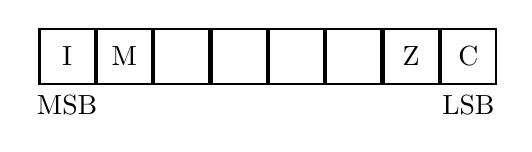
\begin{tikzpicture}
    \tikzstyle{every path}=[thick]
    \edef\turingtapesize{0.7cm}
    \tikzstyle{tmtape}=[draw,minimum size=\turingtapesize]

    \begin{scope}[start chain=1 going right,node distance=0mm]
      \node[on chain=1,tmtape,label=below:MSB] {I};
      \node[on chain=1,tmtape]                 {M};
      \node[on chain=1,tmtape]                 {};
      \node[on chain=1,tmtape]                 {};
      \node[on chain=1,tmtape]                 {};
      \node[on chain=1,tmtape]                 {};
      \node[on chain=1,tmtape]                 {Z};
      \node[on chain=1,tmtape,label=below:LSB] {C};
    \end{scope}
  \end{tikzpicture}
\end{minipage}%
\noindent\begin{minipage}[b]{0.5\linewidth}
  \textbf{C}-Carry Flag\@ \textbf{Z}-Zero Flag\\
  \textbf{I}-Interrupt (1=Enable, 0=Disable)\\
  \textbf{M}-Interrupt Mode (1=Vector, 0=Opcode)
\end{minipage}

\end{appendices}
%TC:endignore
\end{document}
